\chapter{Microservice "Document Analysis"}

\section{Overview}
Document Analysis is a Python microservice that handles document ingestion, semantic entity extraction, vector storage, and natural language response generation. It is a core component of the Contract Central platform, enabling users to query their insurance documents using natural language.

\section{Main Features}
\begin{itemize}
    \item Asynchronous message processing via Google Cloud Pub/Sub
    \item Entity extraction from PDF documents using Gemini 1.5 Pro (VertexAI)
    \item Preparation and flattening of extracted JSON entities
    \item Vector storage and semantic search using ChromaDB
    \item Post-processing with Gemini to generate user-friendly answers
    \item Flask-based API for manual testing and debugging
\end{itemize}

\section{Dependencies}

\subsection{Libraries Used}
\begin{itemize}
    \item \texttt{google-cloud-aiplatform} -- VertexAI SDK for Gemini models
    \item \texttt{google-generativeai} -- Google embedding function for ChromaDB
    \item \texttt{google-cloud-pubsub} -- Pub/Sub messaging system
    \item \texttt{flask} -- Lightweight API framework for local testing
    \item \texttt{chromadb} -- Vector database client
    \item \texttt{pytest} -- Unit testing framework
    \item \texttt{pylint} -- Linter for enforcing code quality
\end{itemize}

\subsection{Custom Modules}
\begin{itemize}
    \item \texttt{extractor.py} -- LLM-based entity extraction
    \item \texttt{prepare\_entities.py} -- Transforms JSON into flat entities
    \item \texttt{operations.py} -- Handles CRUD on the vector database
    \item \texttt{post\_processing.py} -- Natural language response generation
    \item \texttt{entity.py} -- Entity class definition
    \item \texttt{topics.py} -- Message routing logic
    \item \texttt{pubsub\_config.py} -- Pub/Sub client configuration
    \item \texttt{app.py} -- Main Flask app and listener threads
\end{itemize}

\section{Architecture and Workflow}

\subsection{File Upload}
\begin{enumerate}
    \item Triggered via the \texttt{file-upload} Pub/Sub topic.
    \item The file category is extracted from its path.
    \item Gemini extracts structured entities (based on domain-specific prompts).
    \item Entities are flattened and indexed in ChromaDB.
\end{enumerate}

\subsection{Coverage Query}
\begin{enumerate}
    \item Triggered via \texttt{coverage-query} topic.
    \item A semantic search retrieves relevant entities from ChromaDB.
    \item Gemini reformulates a user-facing answer.
    \item The result is published on \texttt{coverage-response}.
\end{enumerate}

\subsection{File Deletion}
\begin{enumerate}
    \item Triggered via \texttt{file-delete}.
    \item All related vectors are deleted from the database.
\end{enumerate}

\section{Endpoints (For Debugging Purpose ONLY)}
\begin{itemize}
    \item \texttt{/create} -- Initialises ChromaDB collection
    \item \texttt{/store} -- Stores hardcoded test file in vector DB
    \item \texttt{/search} -- Performs semantic query using Flask route
    \item \texttt{/delete} -- Deletes entities for given user and file
    \item \texttt{/printdb}, \texttt{/cleandb} -- Debug endpoints to inspect or clean database
\end{itemize}

\section{Testing}

\subsection{Unit Tests}
Tests are located in the \texttt{src/tests/} folder. They cover:
\begin{itemize}
    \item \textbf{extractor}: tests response parsing and LLM call behavior using mocks
    \item \textbf{prepare\_entities}: ensures correct transformation from JSON to Entity
    \item \textbf{entity}: ensures the integrity and representation of the \texttt{Entity} class
\end{itemize}

\subsection{Example:}
\begin{verbatim}
pytest src/tests/
\end{verbatim}

\section{CI/CD Pipeline}

The Document Analysis microservice integrates a continuous integration and deployment (CI/CD) pipeline using GitHub Actions.

\subsection{Automated Tests and Linting}

On every push to the \texttt{main} branch, the pipeline performs the following checks:
\begin{itemize}
    \item Sets up a clean Python 3.10 environment
    \item Installs all dependencies listed in \texttt{requirements.txt}
    \item Runs all unit tests using \texttt{pytest}
    \item Performs static code analysis using \texttt{pylint}, enforcing a minimum score of 8
\end{itemize}

This ensures that the codebase remains stable, maintainable, and compliant with quality standards.

\subsection{Cloud Run Deployment}

Following a successful test and linting stage, the pipeline automatically deploys the latest version of the service to Google Cloud Run.

The deployment script (\texttt{deploy.sh}) builds a Docker image, pushes it to Google Container Registry (\texttt{gcr.io}), and triggers a Cloud Run update with the following specifications:
\begin{itemize}
    \item Service account with restricted permissions for deployment
    \item Custom port configuration (\texttt{5000})
    \item VPC connector for secure access to internal services
    \item Deployment region set to \texttt{europe-west1}
\end{itemize}

This setup enables fully automated and secure delivery from source code to production in less than a minute, with zero manual intervention.

\section{Deployment}

The microservice is deployed using Docker. A script \texttt{deploy.sh} is available to manually deploy the microservice.

\section{Security}
Only messages from authorised users are processed. The system verifies user UIDs before extracting or storing entities. No direct access is allowed to the internal vector database.

In addition, the Document Analysis microservice does not have write access to the Cloud Storage bucket. It can only read PDF documents from pre-authorised URIs for analysis. This ensures that uploaded files remain immutable and protected from unintended modification.

The service also does not store or process any personal user information beyond what is strictly necessary for document analysis. Only the document content, its category, and associated user UUID are referenced during extraction and search. No names, emails, or authentication tokens are accessible to this microservice, thereby minimizing exposure and respecting data minimization principles.

\section{Reactive Use Case Sequence Diagram}

This diagram illustrates the asynchronous flow involved when a user asks a natural language question regarding their insurance coverage. The sequence shows how the backend, Pub/Sub, Document Analysis microservice, ChromaDB, and Gemini interact to generate a response.

\begin{sidewaysfigure}
    \centering
    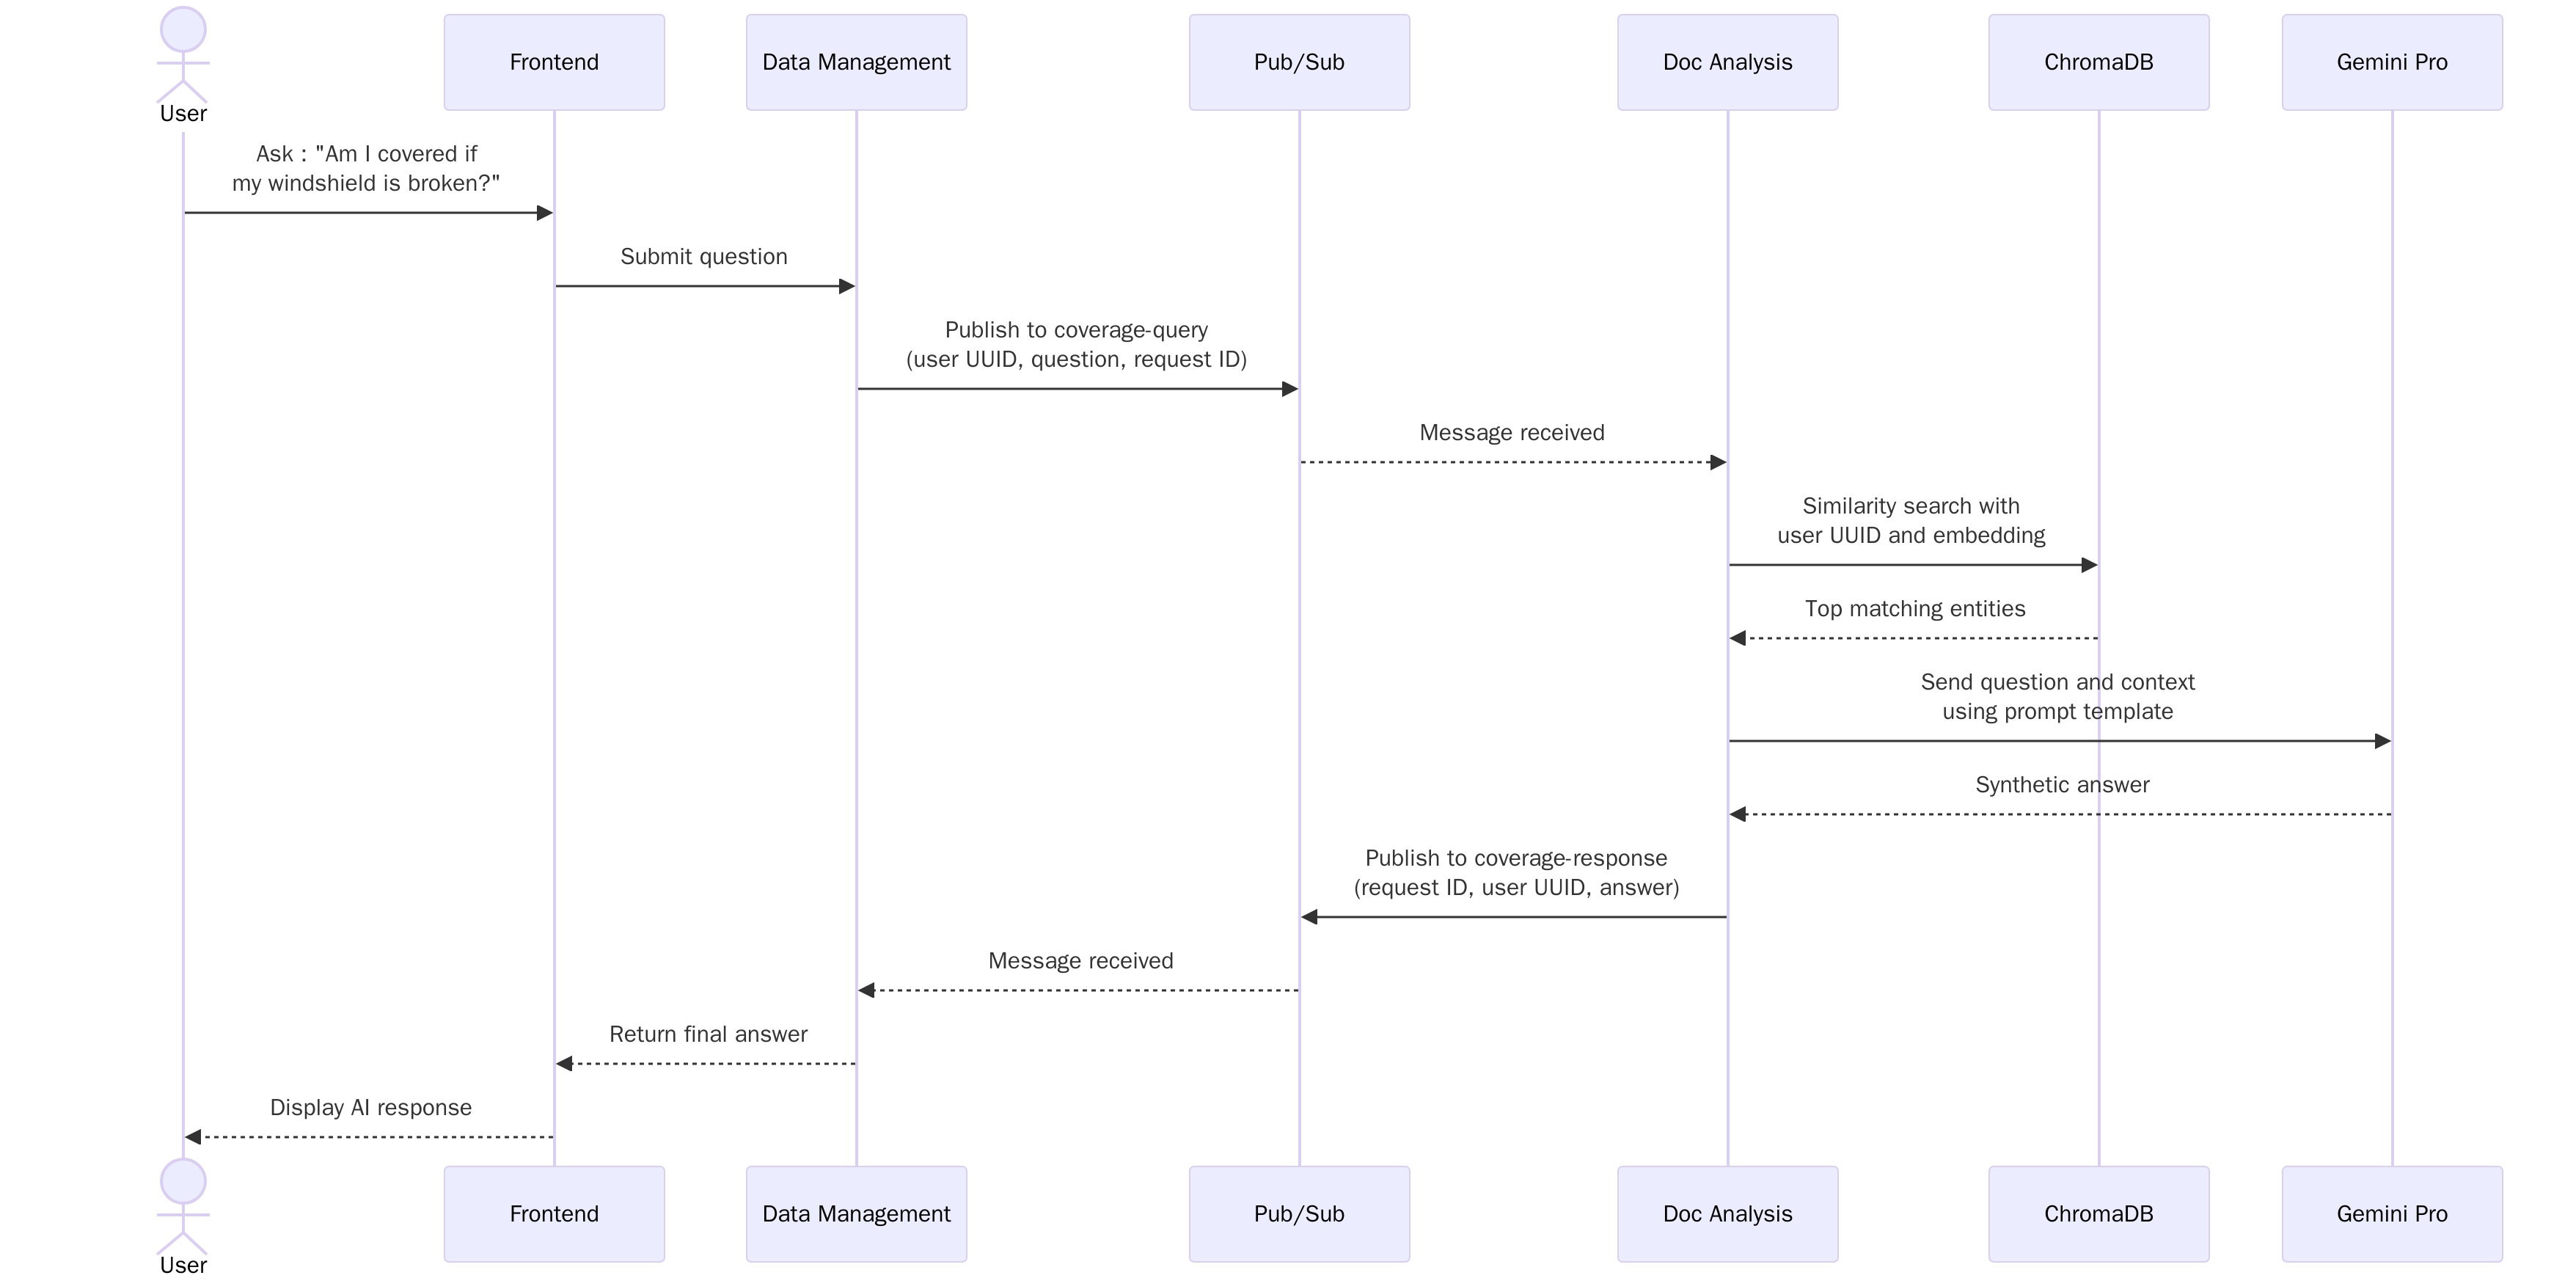
\includegraphics[width=\textheight]{docanalysis/reactive-sequence-diagram.png}
    \caption{Sequence diagram of the reactive use case: question to AI-generated answer}
    \label{fig:sequence-reactive}
\end{sidewaysfigure}
